\documentclass[a4paper,12pt]{article}

%%% Работа с русским языком
\usepackage{cmap}					% поиск в PDF
\usepackage{mathtext} 				% русские буквы в формулах
\usepackage[T2A]{fontenc}			% кодировка
\usepackage[utf8]{inputenc}			% кодировка исходного текста
\usepackage[english,russian]{babel}	% локализация и переносы

%%% Дополнительная работа с математикой
\usepackage{amsfonts,amssymb,amsthm,mathtools} % AMS
\usepackage{amsmath}
\usepackage{unicode-math}
\usepackage{icomma} % "Умная" запятая: $0,2$ --- число, $0, 2$ --- перечисление

\usepackage[left = 2cm, right = 2cm, top = 2cm, bottom = 2cm]{geometry}


%% Номера формул
%\mathtoolsset{showonlyrefs=true} % Показывать номера только у тех формул, на которые есть \eqref{} в тексте.

%% Шрифты
\usepackage{euscript}	 % Шрифт Евклид
\usepackage{mathrsfs} % Красивый матшрифт

%% Свои команды
\DeclareMathOperator{\sgn}{\mathop{sgn}}

%% Перенос знаков в формулах (по Львовскому)
\newcommand*{\hm}[1]{#1\nobreak\discretionary{}
	{\hbox{$\mathsurround=0pt #1$}}{}}

%%% Работа с картинками
\usepackage{graphicx}  % Для вставки рисунков
\graphicspath{{images/}{images2/}}  % папки с картинками
\setlength\fboxsep{3pt} % Отступ рамки \fbox{} от рисунка
\setlength\fboxrule{1pt} % Толщина линий рамки \fbox{}
\usepackage{wrapfig} % Обтекание рисунков и таблиц текстом

%%% Работа с таблицами
\usepackage{array,tabularx,tabulary,booktabs} % Дополнительная работа с таблицами
\usepackage{longtable}  % Длинные таблицы
\usepackage{multirow} % Слияние строк в таблице
\usepackage{upgreek}
\usepackage{enumerate}
\usepackage{ dsfont }

%%% Цветной текст

\usepackage[usenames]{color}
\usepackage{colortbl}

%%% Солнышко

\usepackage[weather]{ifsym}

%%% Гиперссылки

\usepackage{xcolor}
\usepackage{hyperref}
\definecolor{linkcolor}{HTML}{199B03} % цвет ссылок
\definecolor{urlcolor}{HTML}{199B03} % цвет гиперссылок

\hypersetup{pdfstartview=FitH,  linkcolor=linkcolor,urlcolor=urlcolor, colorlinks=true}

\usepackage{minted}

%% Tikz

\usepackage{pgf,tikz,pgfplots}
\pgfplotsset{compat=1.15}
\usepackage{mathrsfs}
\usetikzlibrary{arrows}
\pagestyle{empty}

%%Вставка картинок
\usepackage{graphicx}
\graphicspath{{pictures/}}
\DeclareGraphicsExtensions{.pdf,.png,.jpg}


%% эконометрические сокращения
\def \hb{\hat{\beta}}
\DeclareMathOperator{\sVar}{sVar}
\DeclareMathOperator{\sCov}{sCov}
\DeclareMathOperator{\sCorr}{sCorr}


\def \hs{\hat{s}}
\def \hy{\hat{y}}
\def \hY{\hat{Y}}
\def \he{\hat{\varepsilon}}
\def \v1{\vec{1}}
\def \cN{\mathcal{N}}
\def \e{\varepsilon}
\def \z{z}

\def \hVar{\widehat{\Var}}
\def \hCorr{\widehat{\Corr}}
\def \hCov{\widehat{\Cov}}

\DeclareMathOperator{\tr}{tr}
\DeclareMathOperator*{\plim}{plim}


%% лаг
\renewcommand{\L}{\mathrm{L}}



% DEFS
\def \mbf{\mathbf}
\def \msf{\mathsf}
\def \mbb{\mathbb}
\def \tbf{\textbf}
\def \tsf{\textsf}
\def \ttt{\texttt}
\def \tbb{\textbb}

\def \wh{\widehat}
\def \wt{\widetilde}
\def \ni{\noindent}
\def \ol{\overline}
\def \cd{\cdot}
\def \bl{\bigl}
\def \br{\bigr}
\def \Bl{\Bigl}
\def \Br{\Bigr}
\def \fr{\frac}
\def \bs{\backslash}
\def \lims{\limits}
\def \arg{{\operatorname{arg}}}
\def \dist{{\operatorname{dist}}}
\def \VC{{\operatorname{VCdim}}}
\def \card{{\operatorname{card}}}
\def \sgn{{\operatorname{sign}\,}}
\def \sign{{\operatorname{sign}\,}}
\def \xfs{(x_1,\ldots,x_{n-1})}
\def \Tr{{\operatorname{\mbf{Tr}}}}
\DeclareMathOperator*{\argmin}{arg\,min}
\DeclareMathOperator*{\argmax}{arg\,max}
\DeclareMathOperator*{\amn}{arg\,min}
\DeclareMathOperator*{\amx}{arg\,max}
\def \cov{{\operatorname{Cov}}}
\DeclareMathOperator{\Var}{Var}
\DeclareMathOperator{\Cov}{Cov}
\DeclareMathOperator{\Corr}{Corr}

\def \xfs{(x_1,\ldots,x_{n-1})}
\def \ti{\tilde}
\def \wti{\widetilde}


\def \mL{\mathcal{L}}
\def \mW{\mathcal{W}}
\def \mH{\mathcal{H}}
\def \mC{\mathcal{C}}
\def \mE{\mathcal{E}}
\def \mN{\mathcal{N}}
\def \mA{\mathcal{A}}
\def \mB{\mathcal{B}}
\def \mU{\mathcal{U}}
\def \mV{\mathcal{V}}
\def \mF{\mathcal{F}}

\def \R{\mbb R}
\def \N{\mbb N}
\def \Z{\mbb Z}
\def \P{\mbb{P}}
%\def \p{\mbb{P}}
\def \E{\mbb{E}}
\def \D{\msf{D}}
\def \I{\mbf{I}}

\def \a{\alpha}
\def \b{\beta}
\def \t{\tau}
\def \dt{\delta}
\def \e{\varepsilon}
\def \ga{\gamma}
\def \kp{\varkappa}
\def \la{\lambda}
\def \sg{\sigma}
\def \sgm{\sigma}
\def \tt{\theta}
\def \ve{\varepsilon}
\def \Dt{\Delta}
\def \La{\Lambda}
\def \Sgm{\Sigma}
\def \Sg{\Sigma}
\def \Tt{\Theta}
\def \Om{\Omega}
\def \om{\omega}

%%% Заголовок
\author{Зехов Матвей}
\title{Заметки по многошаговому прогнозированию}
\date{\today}

\begin{document}
\section{ДЗ 1}

\subsection{Номер 1}

\begin{figure}[h]
	
	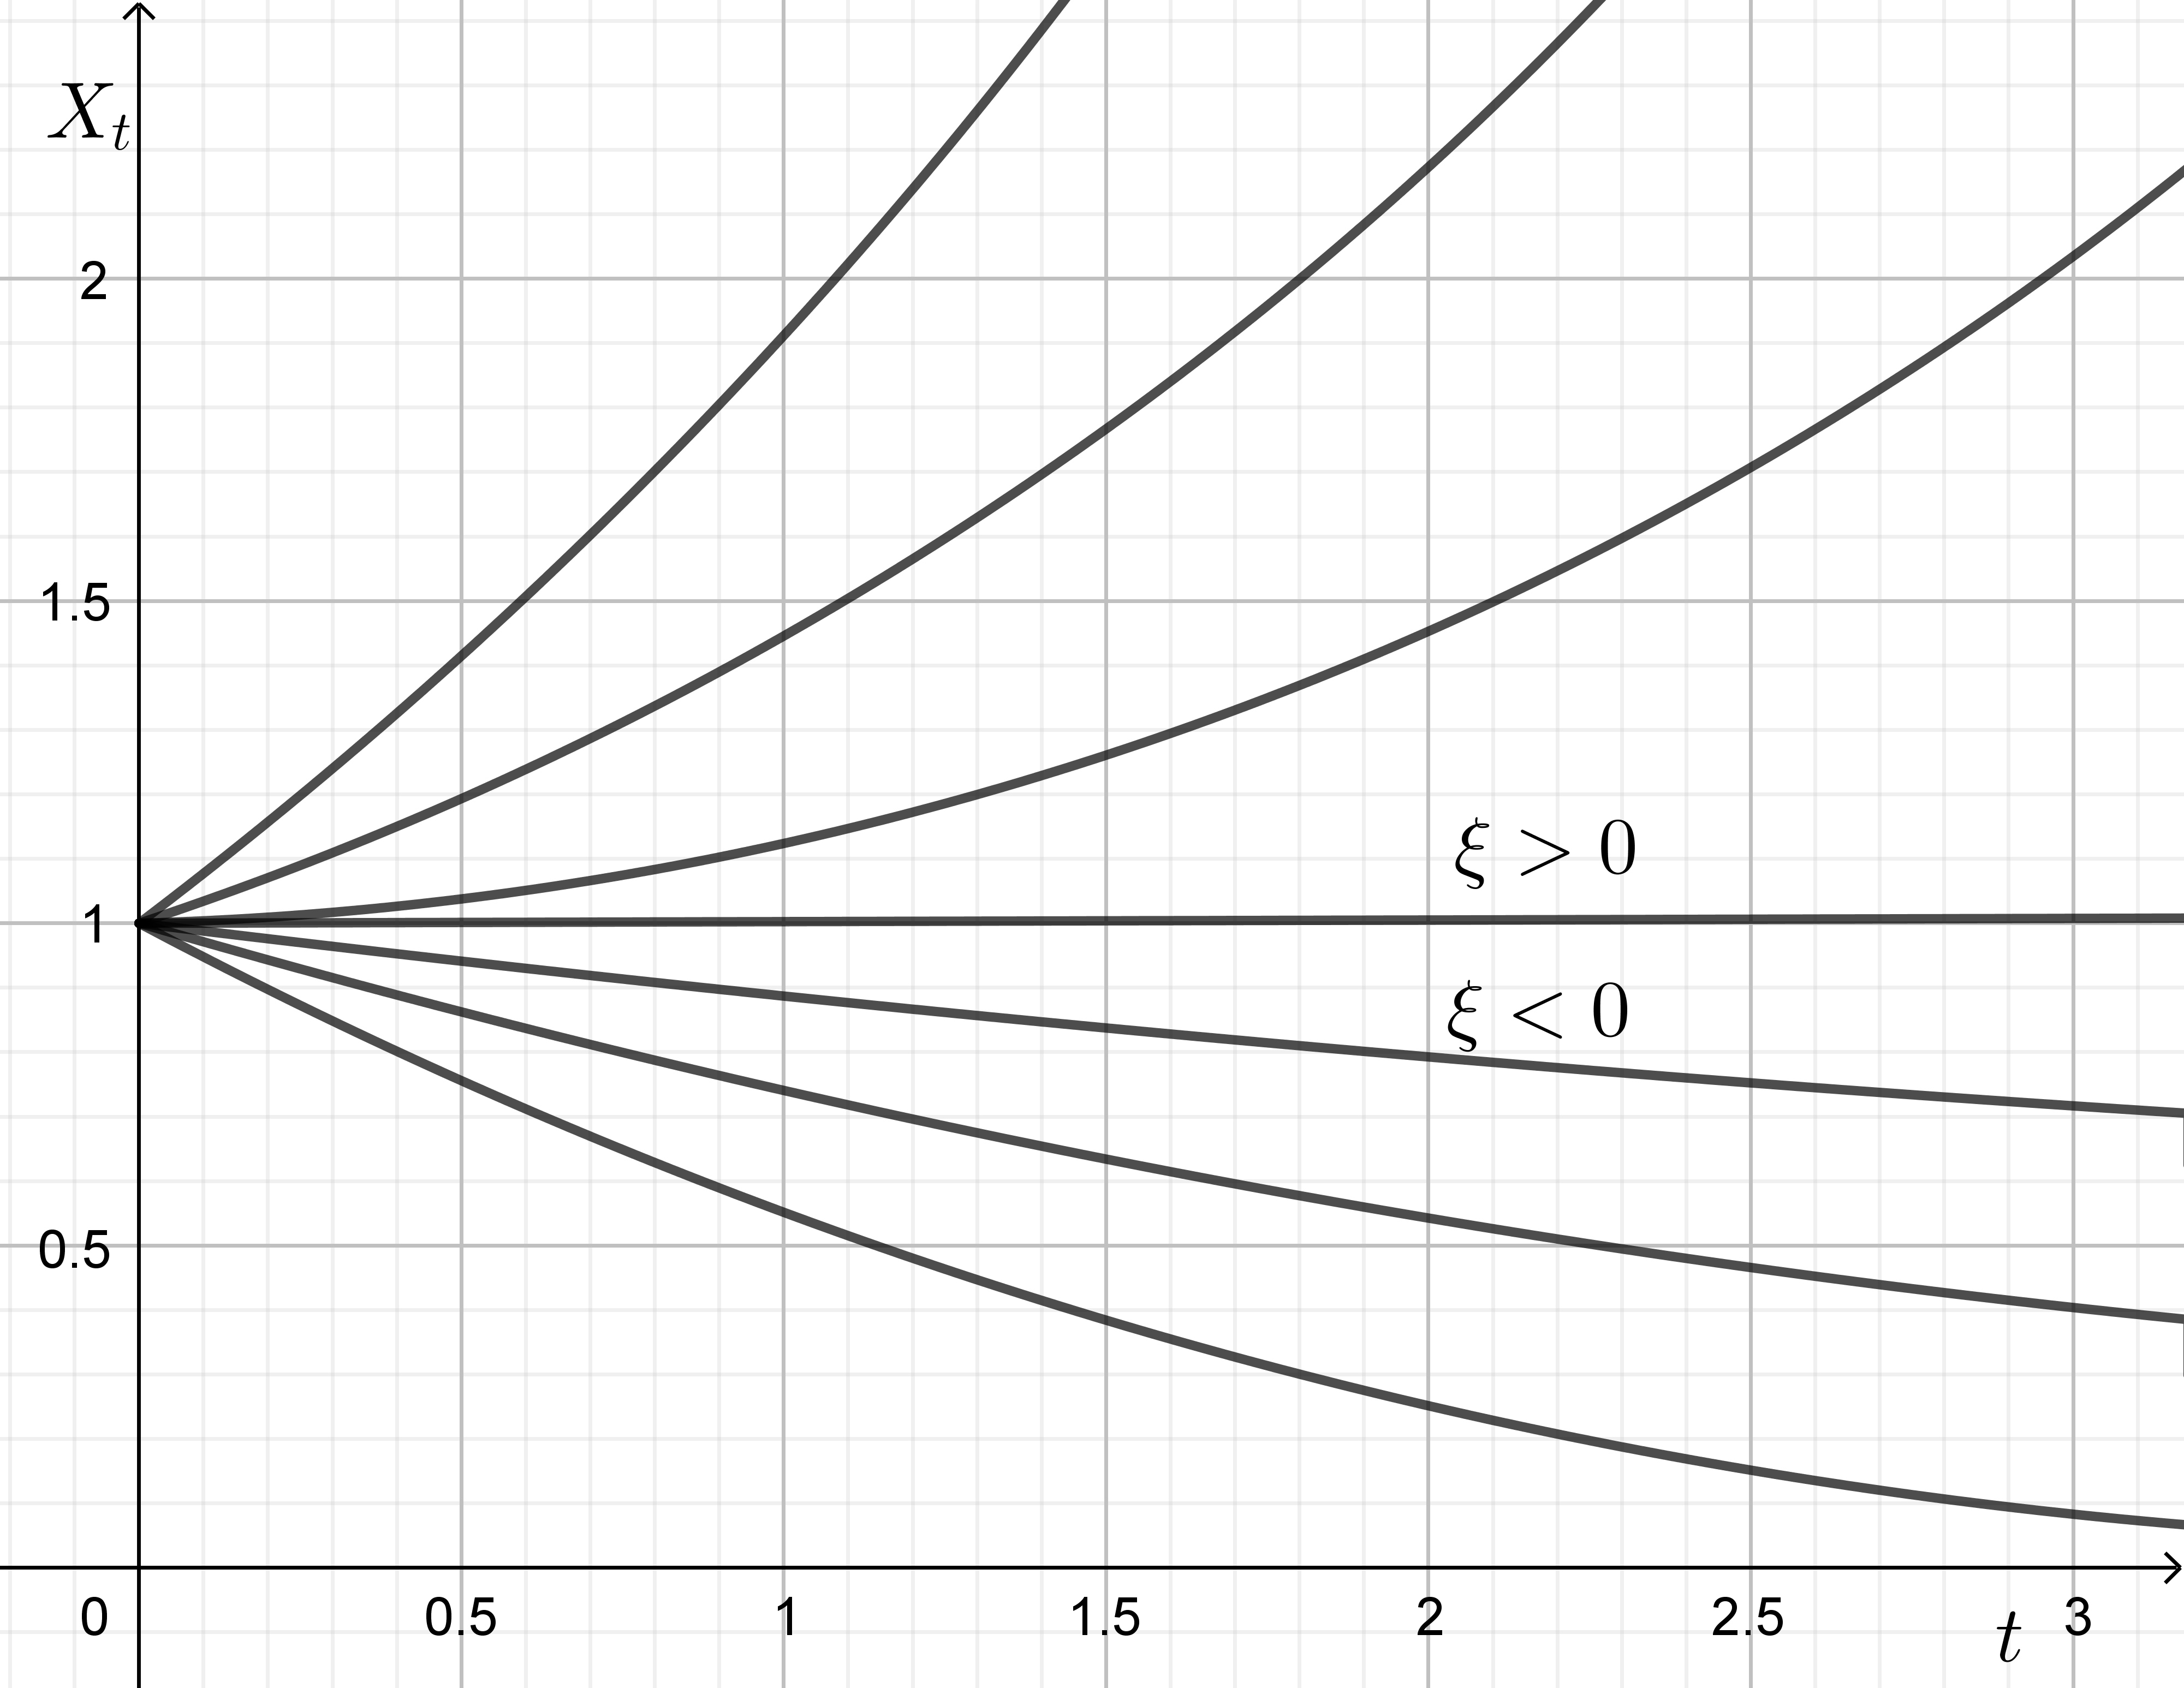
\includegraphics[width = 0.5\linewidth]{11}
	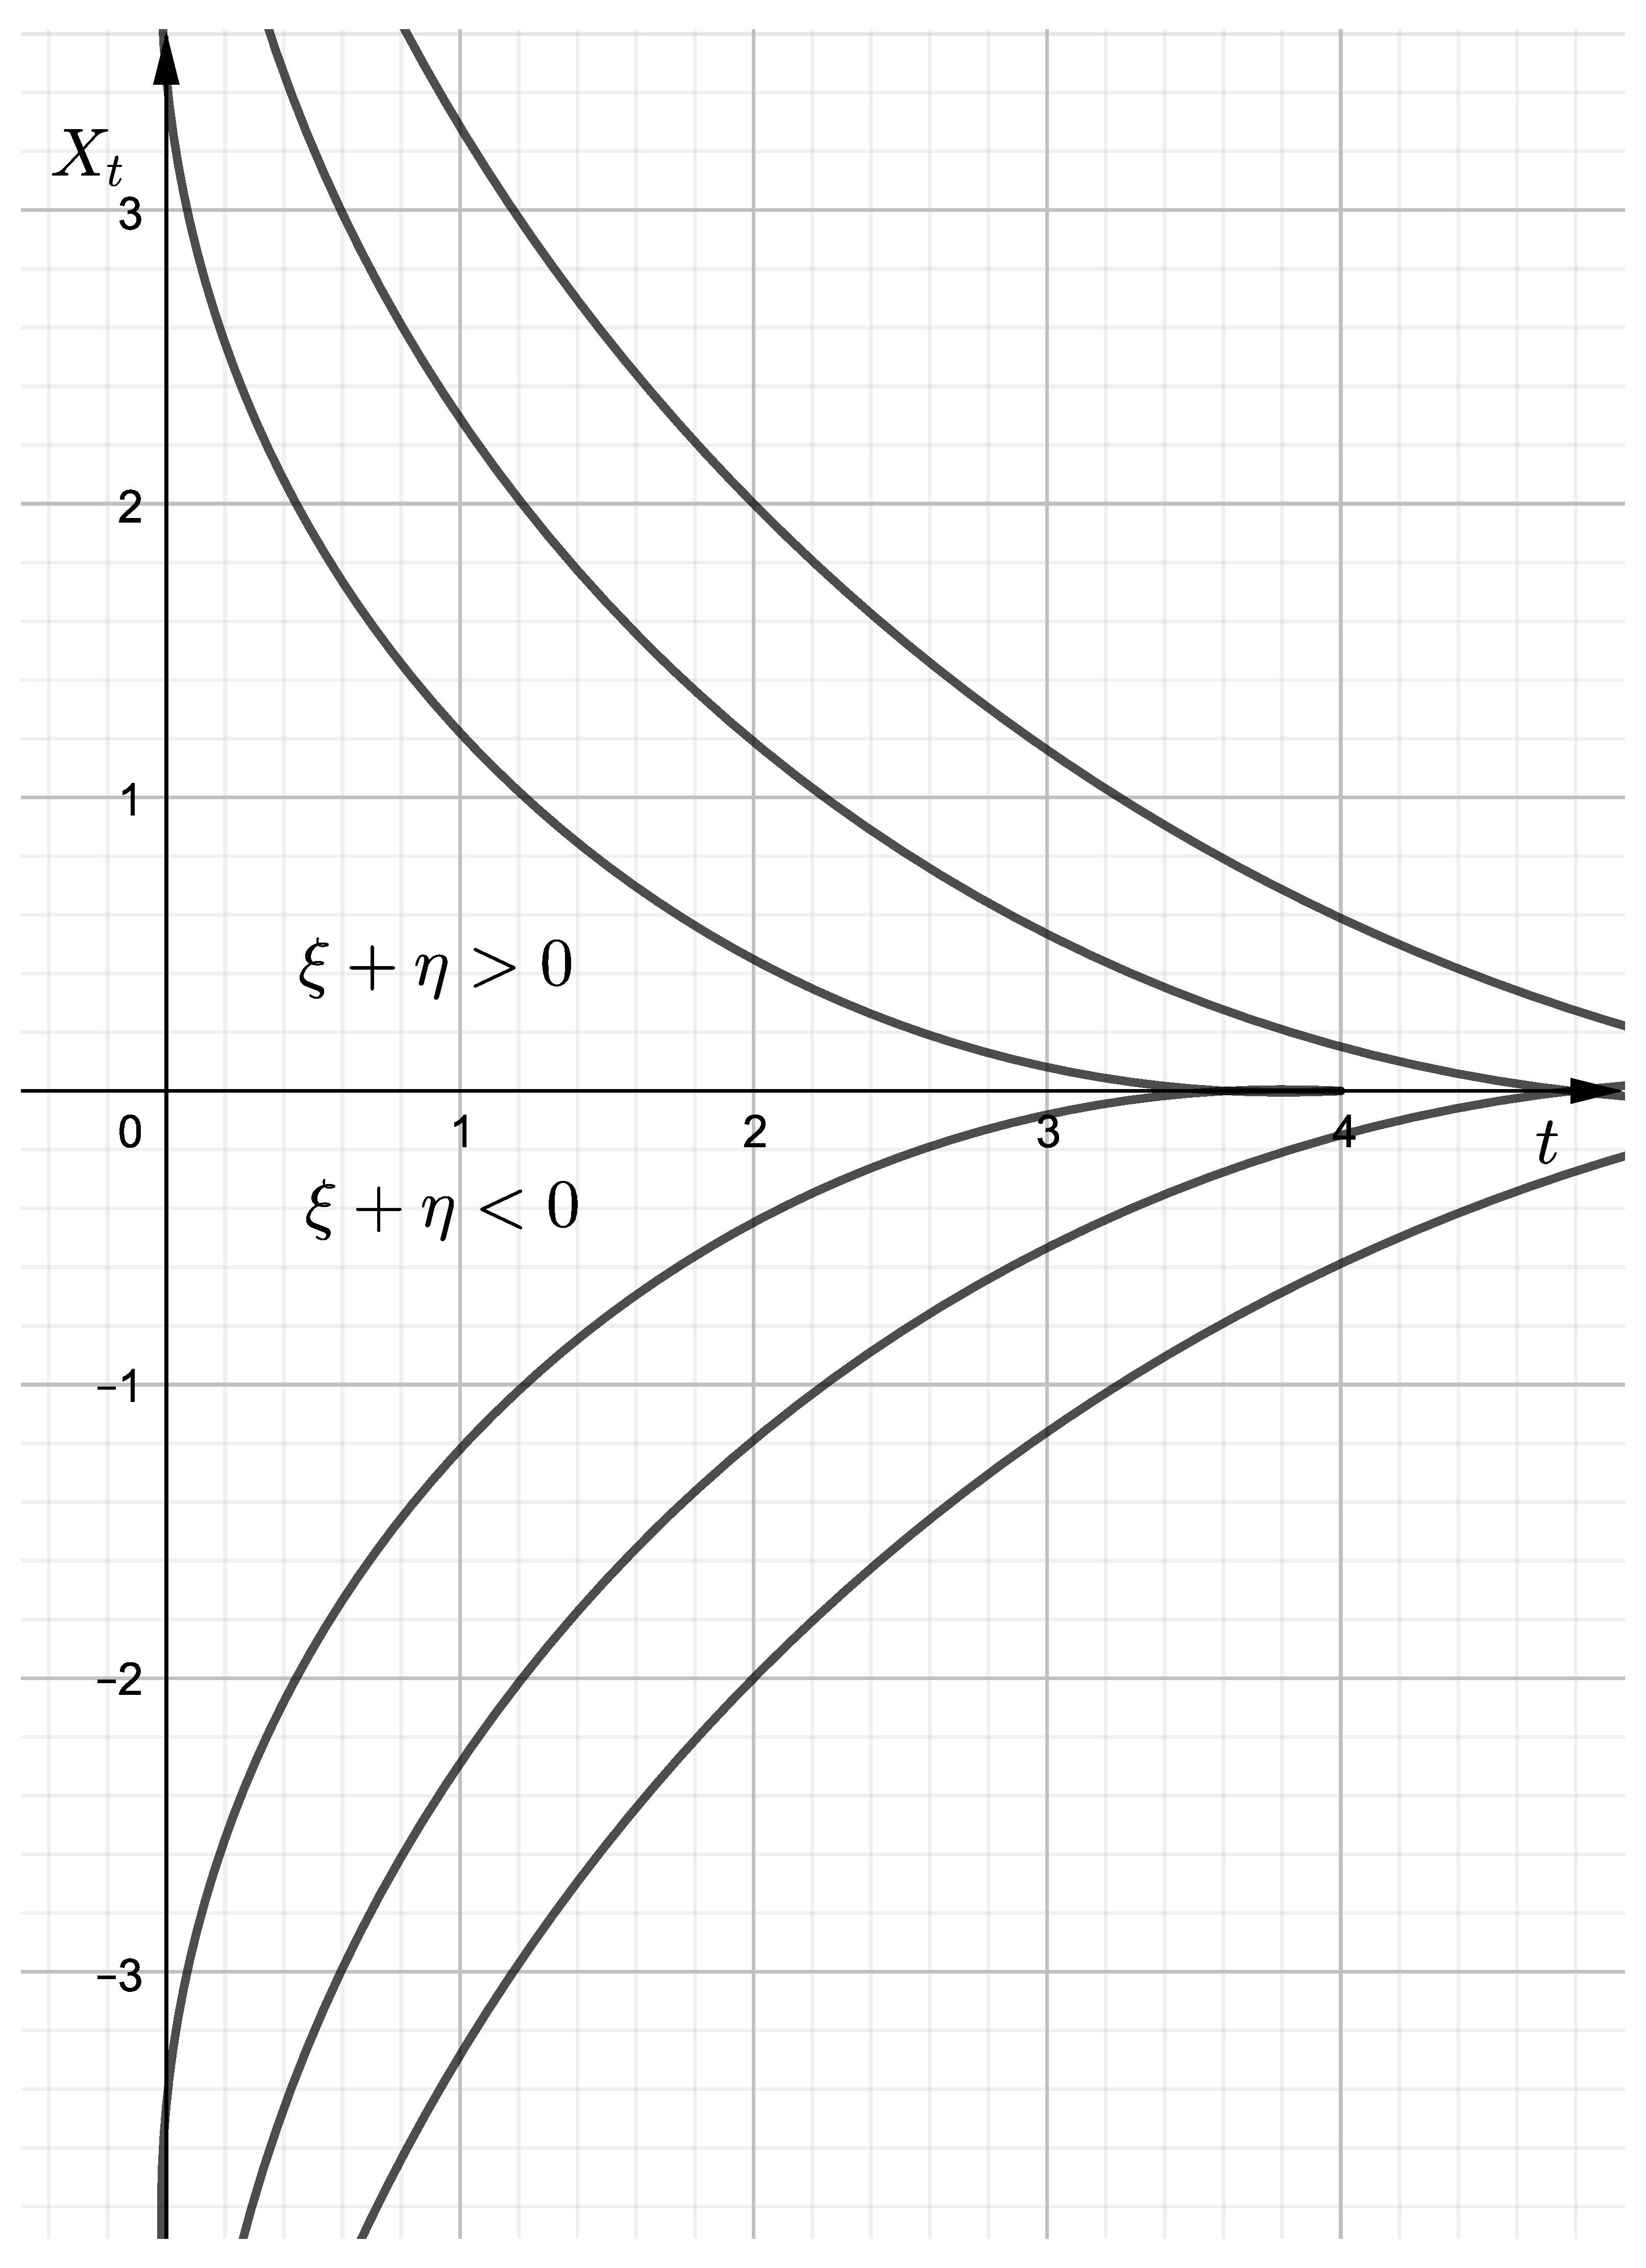
\includegraphics[width = 0.5\linewidth]{12}
	\caption{Траектории}
	\label{traj}
\end{figure}	


\subsubsection{i}
Случайный процесс описан уравнением $ X_{t}=e^{\xi t} $

В зависимости от того, будет реализация случайной величины положительной или отрицательной, кривые будут либо экспоненциально возрастать, либо экспоненциально убывать, где $ \xi $ будет служить коэффициентом скорости роста. Чем ближе $ \xi $ к единице, тем быстрее будет возрастать кривая траектории, а чем ближе к минус единице, тем быстрее убывать. Соответственно, семейство кривых ограничено сверху кривой $ X_t = e^\xi $, а снизу -- кривой   $ X_t = e^{-\xi} $. Графики возможных траекторий можно увидеть на Рис. \ref{traj} слева.

\subsubsection{ii}
Случайный процесс описан уравнением $X_{t}=(\xi+\eta) / t$. В зависимости от того, будет ли реализация случайной величины $ \xi + \eta $ положительной или отрицательной, траекториями будут семейства гипербол. Соответственно, чем ближе к нулю будет реализована данная случайная величина, тем более вогнуты будут гиперболы вогнуты в сторону точки (0.0). Графики возможных траекторий можно увидеть на Рис. \ref{traj} справа.
\subsection{Номер 2}

\[ P\{X_{t_1} < X_{t_2}\} = P\{t_1(\xi_1 + \alpha(\xi_2 + 2\alpha))<t_1(\xi_1 + \alpha(\xi_2 + 2\alpha)) \}=  \]
\[
P\{ (t_1 - t_2)\xi_1 + (t_1 - t_2)\alpha \xi_2 < (t_2 - t_1)2\alpha^2\} = \\P\{ \xi_1 + \alpha\xi_2 \ge -2\alpha^2\} = P\{ \xi_1 + \alpha\xi_2 + 2\alpha^2 \ge 0\} = 1\]
	
	
Чтобы вероятность того, что эта случайная величина была положительной стала равной единице, рассмотрим график. Так как указано, что параметр $ \alpha $ является реальным числом, будем рассматривать только случаи с положительным дискриминантом. Чтобы учесть максимальное количество случаев, при которых значение функции в точке положительно, максимально "опустим" параболу, максимизировав дискриминант. Очевидно, что это произойдёт в двух точках относительно $ \xi $: (1, -1), (-1, -1)

\[ D = \xi_2^2 - 8\xi_1 \]

\[ \alpha_1 = \frac{-\xi_2 - \sqrt{\xi_2^2 - 8\xi_1}}{4} \]

\[ \alpha_1 = \frac{-\xi_2 + \sqrt{\xi_2^2 - 8\xi_1}}{4} \]


Все мозможные случаи корней при $ \xi_2 = +- 1 $:
\[ 
\begin{cases}
	\alpha_{11} = -\frac{1}{2}\\
	\alpha_{12} = -1\\
	\alpha_{21} = \frac{1}{2}\\
	\alpha_{22} = 1
\end{cases}
 \]

Следовательно, взяв значения параметра $ \alpha \in [-1, 1] $, парабола будет гарантированно будет принимать положительные значения.
Ответ:  $ \alpha \in [-1, 1] $

\subsection{Задача 3}

\[  f _ { z } ( x ) = \frac { 1 } { 2 } e ^ { - x } + e ^ { - 2 x } , x > 0  \]

\begin{equation}
\begin{aligned}  L [ p ] ( u ) = \int _ { 0 } ^ { \infty } \left( \frac { 1 } { 2 } e ^ { - x } + e ^ { - 2 x } \right) e ^ { - u x } d x  = \int _ { 0 } ^ { \infty } \frac { 1 } { 2 } e ^ { - x ( 1 + u ) } + e ^ { - x ( 2 + u ) } d x = \\ = \frac { 1 } { 2 ( 1 + u ) } + \frac { 1 } { 2 + u } = \frac { 2 + u + 2 + 2 u } { 4 + 4 u + 2 u + 2 u ^ { 2 } } =  \frac { 4 + 3 u } { 2 u ^ { 2 } + 6 u + 4 } \end{aligned}
\end{equation}

\begin{equation}
\begin{aligned}
L [ U ] ( u ) = \frac { \frac { 4 + 3 u } { 2 u ^ { 2 } + 6 u + 4 } } { u \left( 1 - \frac { 4 + 3 u } { 2 u ^ { 2 } + 6 u + 4 } \right) } = \frac { \frac { 4 + 3 u } { 2 u ^ { 2 } + 6 u + 4 } } { u \left( \frac { 2 u ^ { 2 } + 3 u } { 2 u ^ { 2 } + 6 u + 4 } \right) }= \frac { 3 u + 4 } { 2 u ^ { 3 } + 3 u ^ { 2 } } = \frac { 3 u  + 4 } { u ^ { 2 } ( 2 u + 3 ) } 
\end{aligned}
\end{equation}




\[ 
\frac { 3 u + 4 } { u ^ { 2 } ( 2 u + 3 ) } = \frac { A } { u } + \frac { B } { u ^ { 2 } } + \frac { C } { u + 3 }  = \frac { A u ( 2 u + 3 ) + B ( 2 u + 3 ) + C u ^ { 2 } } { u ^ { 2 } ( 2 u + 3 ) } = \frac { 2 A u ^ { 2 } + C u ^ { 2 } + 3 A u + 2 B u + 3 B } { u ^ { 2 } ( 2 u + 3 ) }
 \]

\begin{equation}
\left\{ \begin{array} { l } { C + 2 A = 0 } \\ { 3 A + 2 B = 3 } \\ { 3 B = 4 } \end{array} \Rightarrow \left\{ \begin{array} { l } { A = \frac { 1 } { 9 } } \\ { B = \frac { 4 } { 3 } } \\ { C = - \frac { 2 } { 9 } } \end{array} \right. \right.
\end{equation}


\[ U(t) = \frac{1}{9} + \frac{4}{3}t - \frac{1}{9}\exp^{-\frac{3}{2}t}\]

\subsection{Задача 4}
\subsubsection{i}

 \begin{wrapfigure}{l}{0.4\textwidth}
	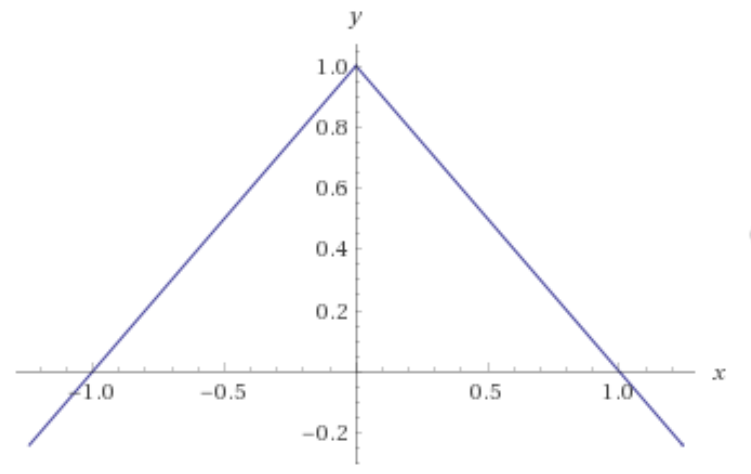
\includegraphics[width=\linewidth]{13}
	\caption{$  f_{\xi - \eta}(x) $}
	\label{minmax}
\end{wrapfigure}


Для начала выведем несколько необходимых свойств функций плотностей.
\begin{equation}
\begin{aligned}
	F_{|\xi|} = P\{|\xi| \le x\}  = P\{-x \le \xi \le x \} =\\ P\{\xi \le x \} - P\{\xi \le -x \} = F_\xi(x) - F_\xi(-x) 
\end{aligned}
\end{equation}
Следовательно:
 \[ f_{|\xi|}(x) = f_\xi(x) + f_\xi(-x) \] 
 
 Теперь по формуле свёртки выведем следующую плотность:
 
 \[ f_{\xi - \eta}(x) = f_{\xi + (-\eta)}(x) \]
 
Для этого выведем следующее свойство:

 
\[  F_{-\eta}(x) = P\{-\eta \le x\} = P\{\eta \ge -x\} =\\ 1 -F_{\eta}(-x) \Rightarrow f_{-\eta}(x) = f_{\eta}(-x) \] 

Теперь возьмём интеграл:


\[  f_{\xi - \eta}(x) = \int_{-\infty}^{\infty} I\{u - x \in [0;1]\} I\{- x \in [0;1]\} = \int_{max(u-1,-1)}^{min(u,0)}1 dx = min(u,0) - max(u-1,-1) \]

Полученная фукнция изображена на \ref{minmax}.

Так как функция симметричная, $ f_{|\xi|}(x) = f_\xi(x) + f_\xi(-x) = 2 f_\xi(x) $. Следовательно: 

\[  f_{|\xi - \eta|}(x) = 2(min(u,0) - max(u-1,-1))  \]

Данная функция не удовлетворяет стандартным условиям, накладываемым на функции плотности. Ситуацию исправит нормированная константа $ \frac{1}{2} $. Следовательно, ответ:

\[  f_{|\xi - \eta|}(x) = min(u,0) - max(u-1,-1) \]

\subsubsection{ii}

По формуле свёртки:
\begin{equation*}
\begin{aligned}
f_{\xi + \eta} = \int_{-\infty}^{\infty} \frac{1}{4} \exp^{-|u-x|-|x|} dx=  \frac{1}{4}  \left( \int_{-\infty}^{0} \exp^{-|u-x|+x} dx + \int_{0}^{\infty}  \exp^{-|u-x|-x} dx \right) = \\ \frac{1}{4} \left( \int_{-\infty}^{min(u,0)} \exp^{-u+2x} dx+ \int_{min(u,0)}^{0} \exp^{u} dx+ \int_{0}^{max(u,0)}  \exp^{-u} dx + \int_{max(u,0)}^{+\infty}  \exp^{u-2x} dx \right) = \\
\frac{1}{4} \left( \frac{1}{2}\exp^{-u+2x} \Biggr|_{-\infty}^{min(u,0)}  + x \exp^u \Biggr|_{min(u,0)}^{0} + x \exp^{-u} \Biggr|_{0}^{max(u, 0)}  - \frac{1}{2} \exp^{u-2x} \Biggr|_{max(u, 0)}^{+\infty} \right) = \\
\frac{1}{4} \left( \frac{1}{2}\exp^{-u+2min(u,0)} - min(u,0) \exp^u + max(u,0) \exp^{-u} + \frac{1}{2} \exp^{u-2max(u, 0)} \right)
\end{aligned}
\end{equation*}

Вольфрам сказал, что интеграл под этой функцией равен единице, так что всё должно быть верно. По форме распределение напоминает нормальное. Касательно возникших функций минимума и максимума, они призваны регулировать функцию в зависимости от знака параметра $ u $. В зависимости от него один из четырёх интегралов во 2 строке будет схлопываться в нулевой.

\subsection{Задача 5}

\subsubsection{i}

Нет, не является процессом восстановления, так как $ p\{ \xi_i \ge 0 \} \neq 1 $

\subsubsection{ii}
Каждая траектория имеед вид ломаной кривой. Она начинается в точке ноль и образует один из путей (слева направо) в древовидной структуре на Рис.  \ref{rombs}.Для примера одна из возможных траекторий окрашена в оранжевый. Данная фигура по виду очень напоминает треугольник Паскаля.


\begin{figure}[h]
	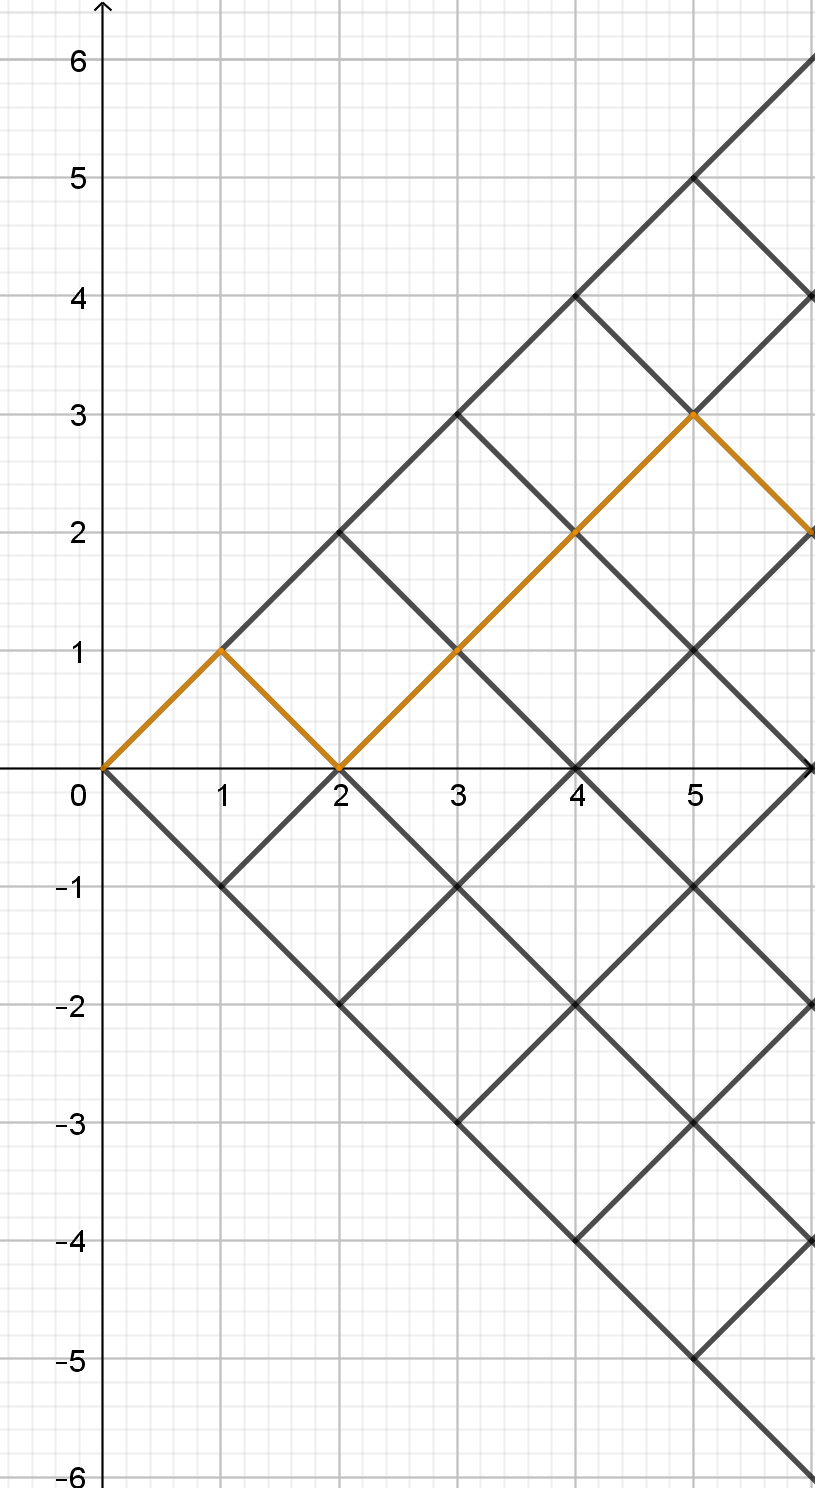
\includegraphics[width=0.3\linewidth]{14}
	\caption{Траектории $ S_n $}
	\label{rombs}
\end{figure}
\subsubsection{iii}
\subsubsection{iv}

\subsection{Задача 6}

\[ \{S_n \ge t \} = \{ S_n > t \} \cup \{ S_n = t \} = \]

Так как $\left\{S_{n}>t\right\}=\left\{N_{t}<n\right\}$ 

\[  = \left\{N_{t}<n\right\} \cup \{ S_n = t \}  = \]

Так как функция $ N_t $ непрерывна справа, то по построению очевидно, что $  \{ S_n = t \} = \left\{N_{t}=n\right\}  $

\[ = \left\{N_{t}<n\right\} \cup  \left\{N_{t}=n\right\} = \left\{N_{t}\le n\right\}\]

\end{document}
